% ====================================================================
%  RQ1 -- Uncertainty (Chapter 3, ~6 min)
%  Layout convention: text/maths left, figure right.
% ====================================================================

\roadmapframe{1}{RQ1. How can machine learning models, and deep survival models in particular, quantify uncertainty in individual predictions?}

\begin{frame}{Why uncertainty? Refer unsure cases}
\begin{columns}[c]
  \begin{column}{0.53\textwidth}
    \small
    \textbf{Two kinds of uncertainty}
    \begin{itemize}
      \item \textbf{Aleatoric} -- noise in the data: $p(y \mid \bm{x}, \bm{\theta})$
      \item \textbf{Epistemic} -- what the model does not know: $p(\bm{\theta} \mid \D)$
    \end{itemize}
    \vspace{0.3em}
    \textbf{Bayesian posterior predictive}
    \[
      p(y \mid \bm{x}, \D) = \int p(y \mid \bm{x}, \bm{\theta})\, p(\bm{\theta} \mid \D)\, \d\bm{\theta}
    \]
    \vspace{-0.3em}
    Intractable for neural nets $\rightarrow$ approximate.

    \vspace{0.4em}
    Use: if the uncertainty exceeds a threshold, refer the case to a clinician.
  \end{column}
  \begin{column}{0.45\textwidth}
    \centering
    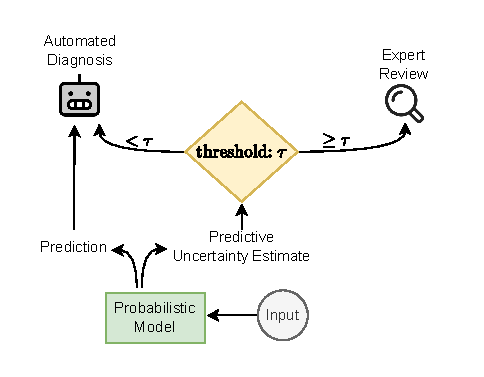
\includegraphics[width=\linewidth]{diagnosis_pipeline.pdf}
    \figsource{Figure adapted from Filos et al.~\cite{filos2019systematic}}
  \end{column}
\end{columns}
\end{frame}

\begin{frame}{BaySurv: three probabilistic variants}
\begin{columns}[c]
  \begin{column}{0.56\textwidth}
    \small
    \textbf{Shared setup.} The risk score is a Gaussian $\N(\mu_{\bm{x}}, \sigma^2_{\bm{x}})$; each sample gives one survival curve.

    \vspace{0.9em}
    \textbf{VI.} A distribution per weight \cite{blundell2015weight} -- twice the parameters.

    \vspace{0.9em}
    \textbf{MC dropout.} Dropout stays on at prediction time \cite{gal_dropout_2016} -- same size as a normal network.

    \vspace{0.9em}
    \textbf{SNGP.} A Gaussian-process output layer \cite{liu2020simple} -- no sampling.
  \end{column}
  \begin{column}{0.42\textwidth}
    \centering
    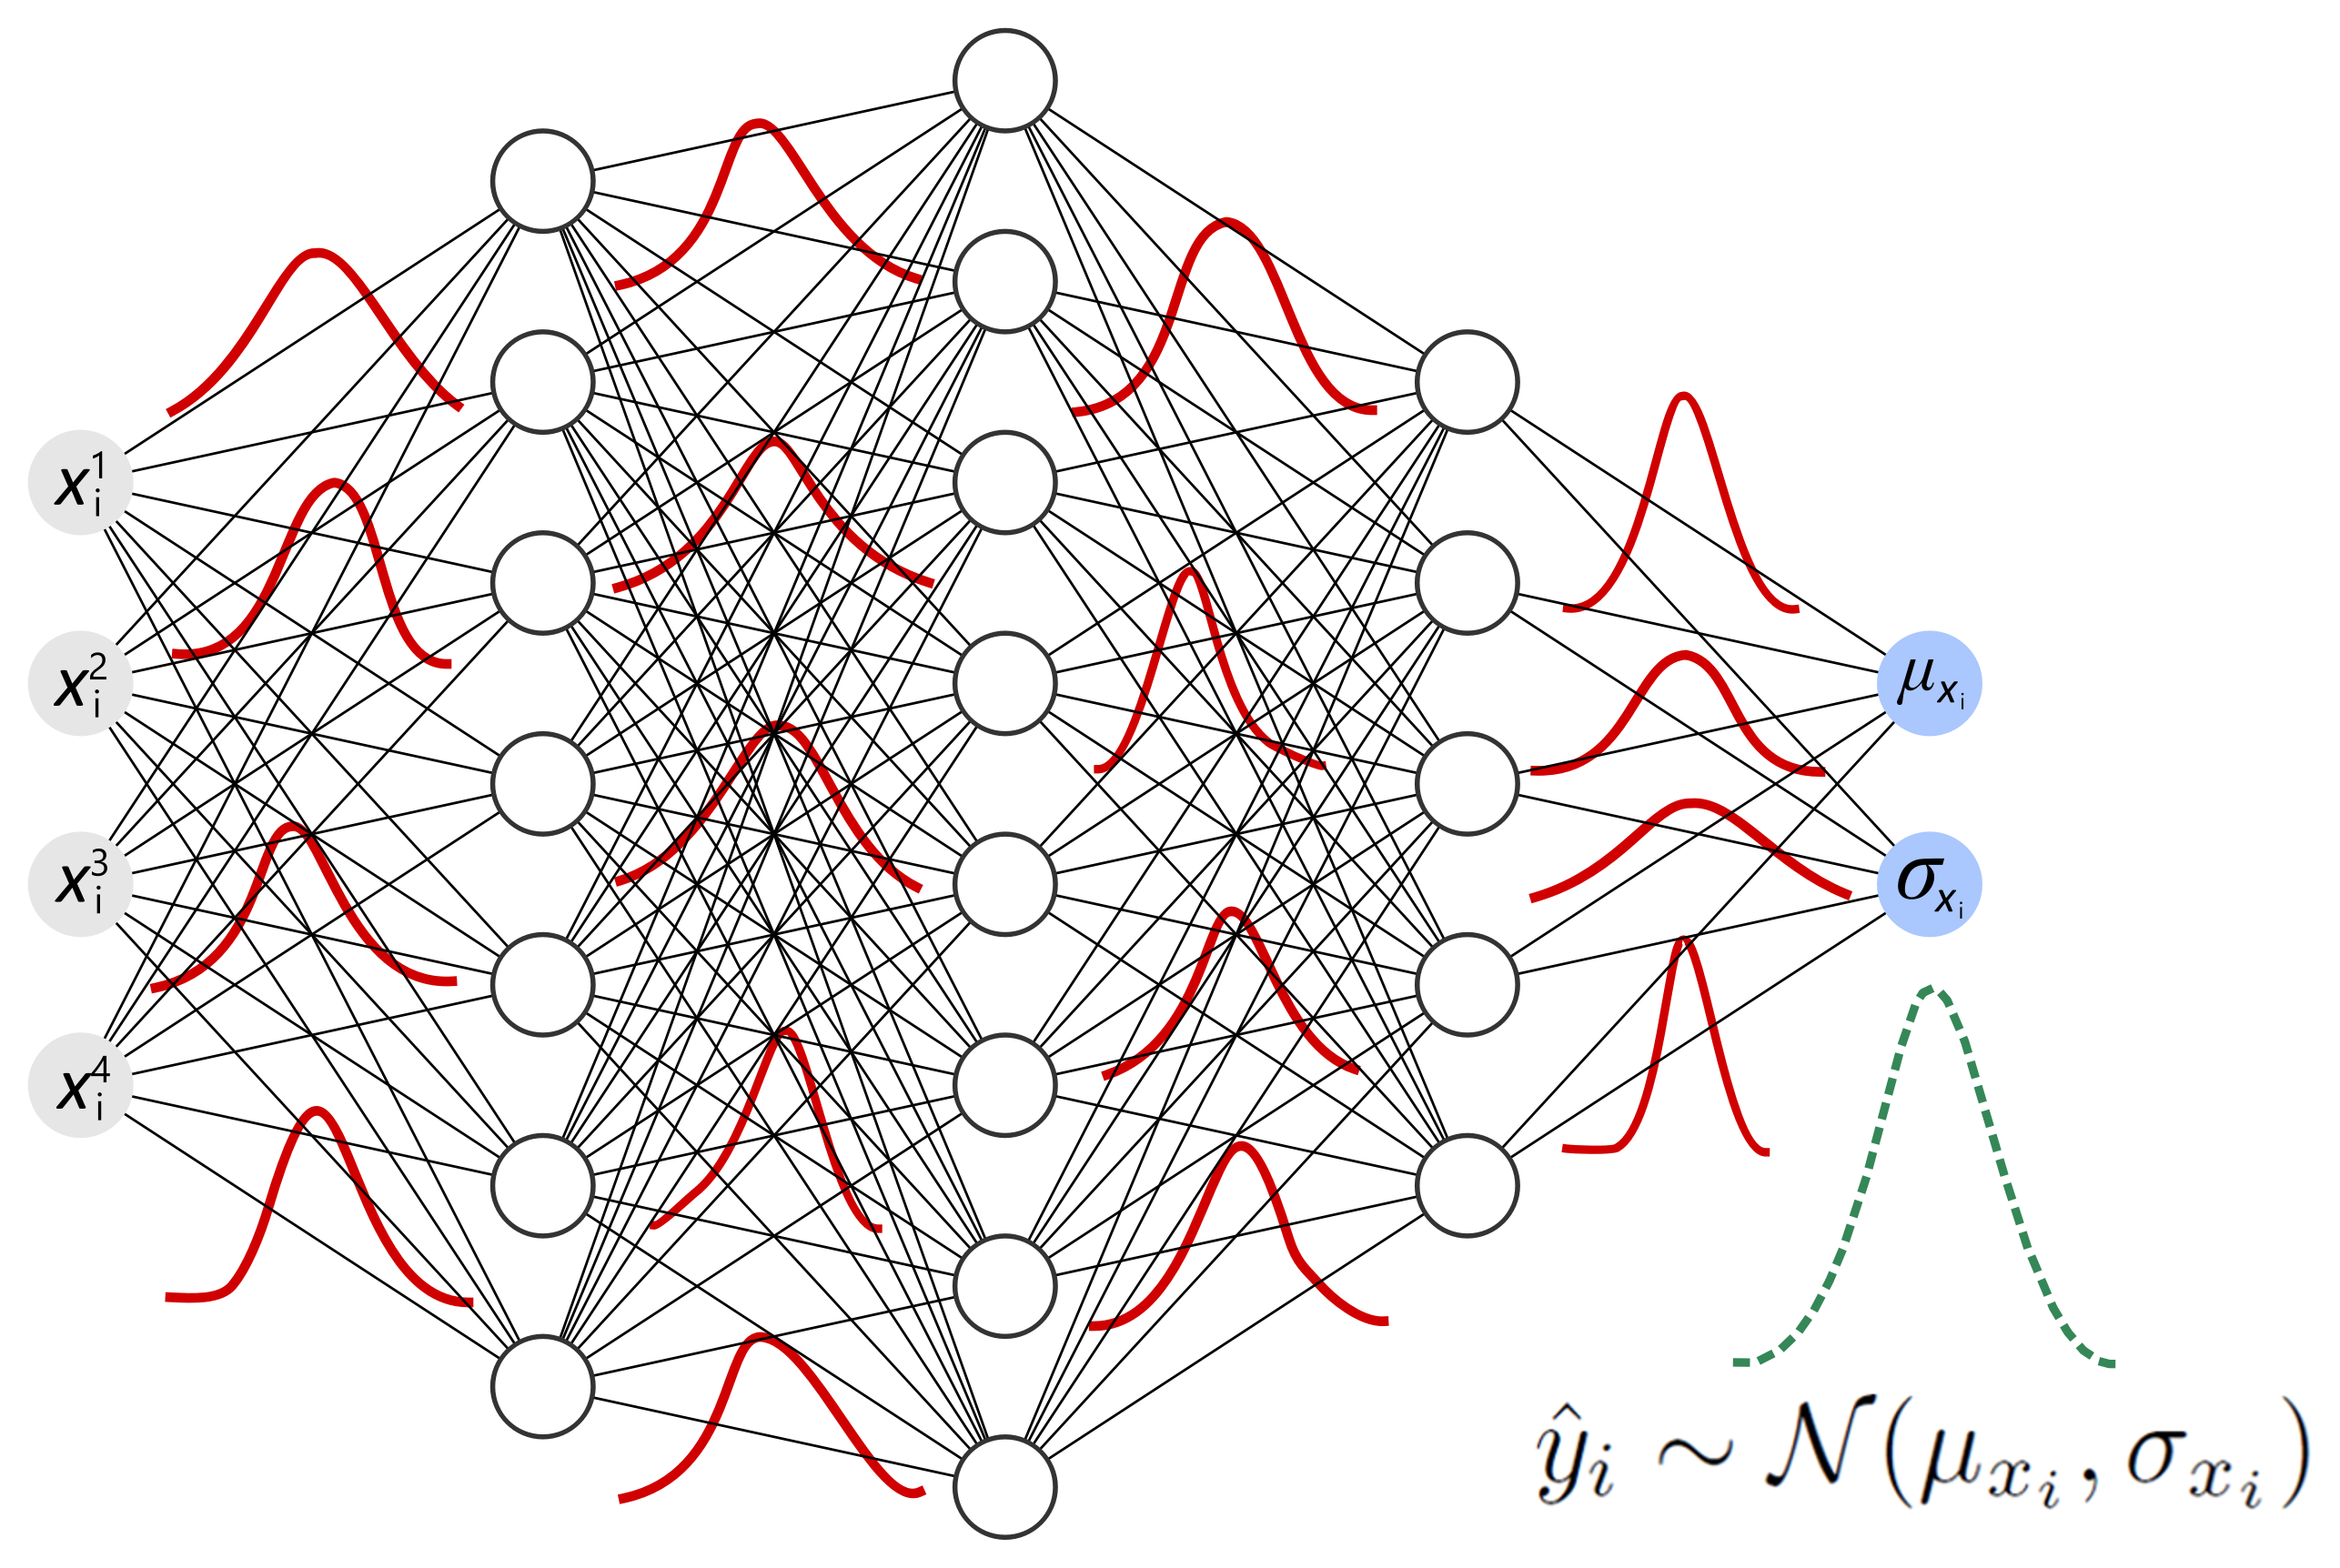
\includegraphics[width=0.7\linewidth]{baysurv_vi.png}\\[-0.2em]
    {\scriptsize\textbf{VI.}}\\[0.2em]
    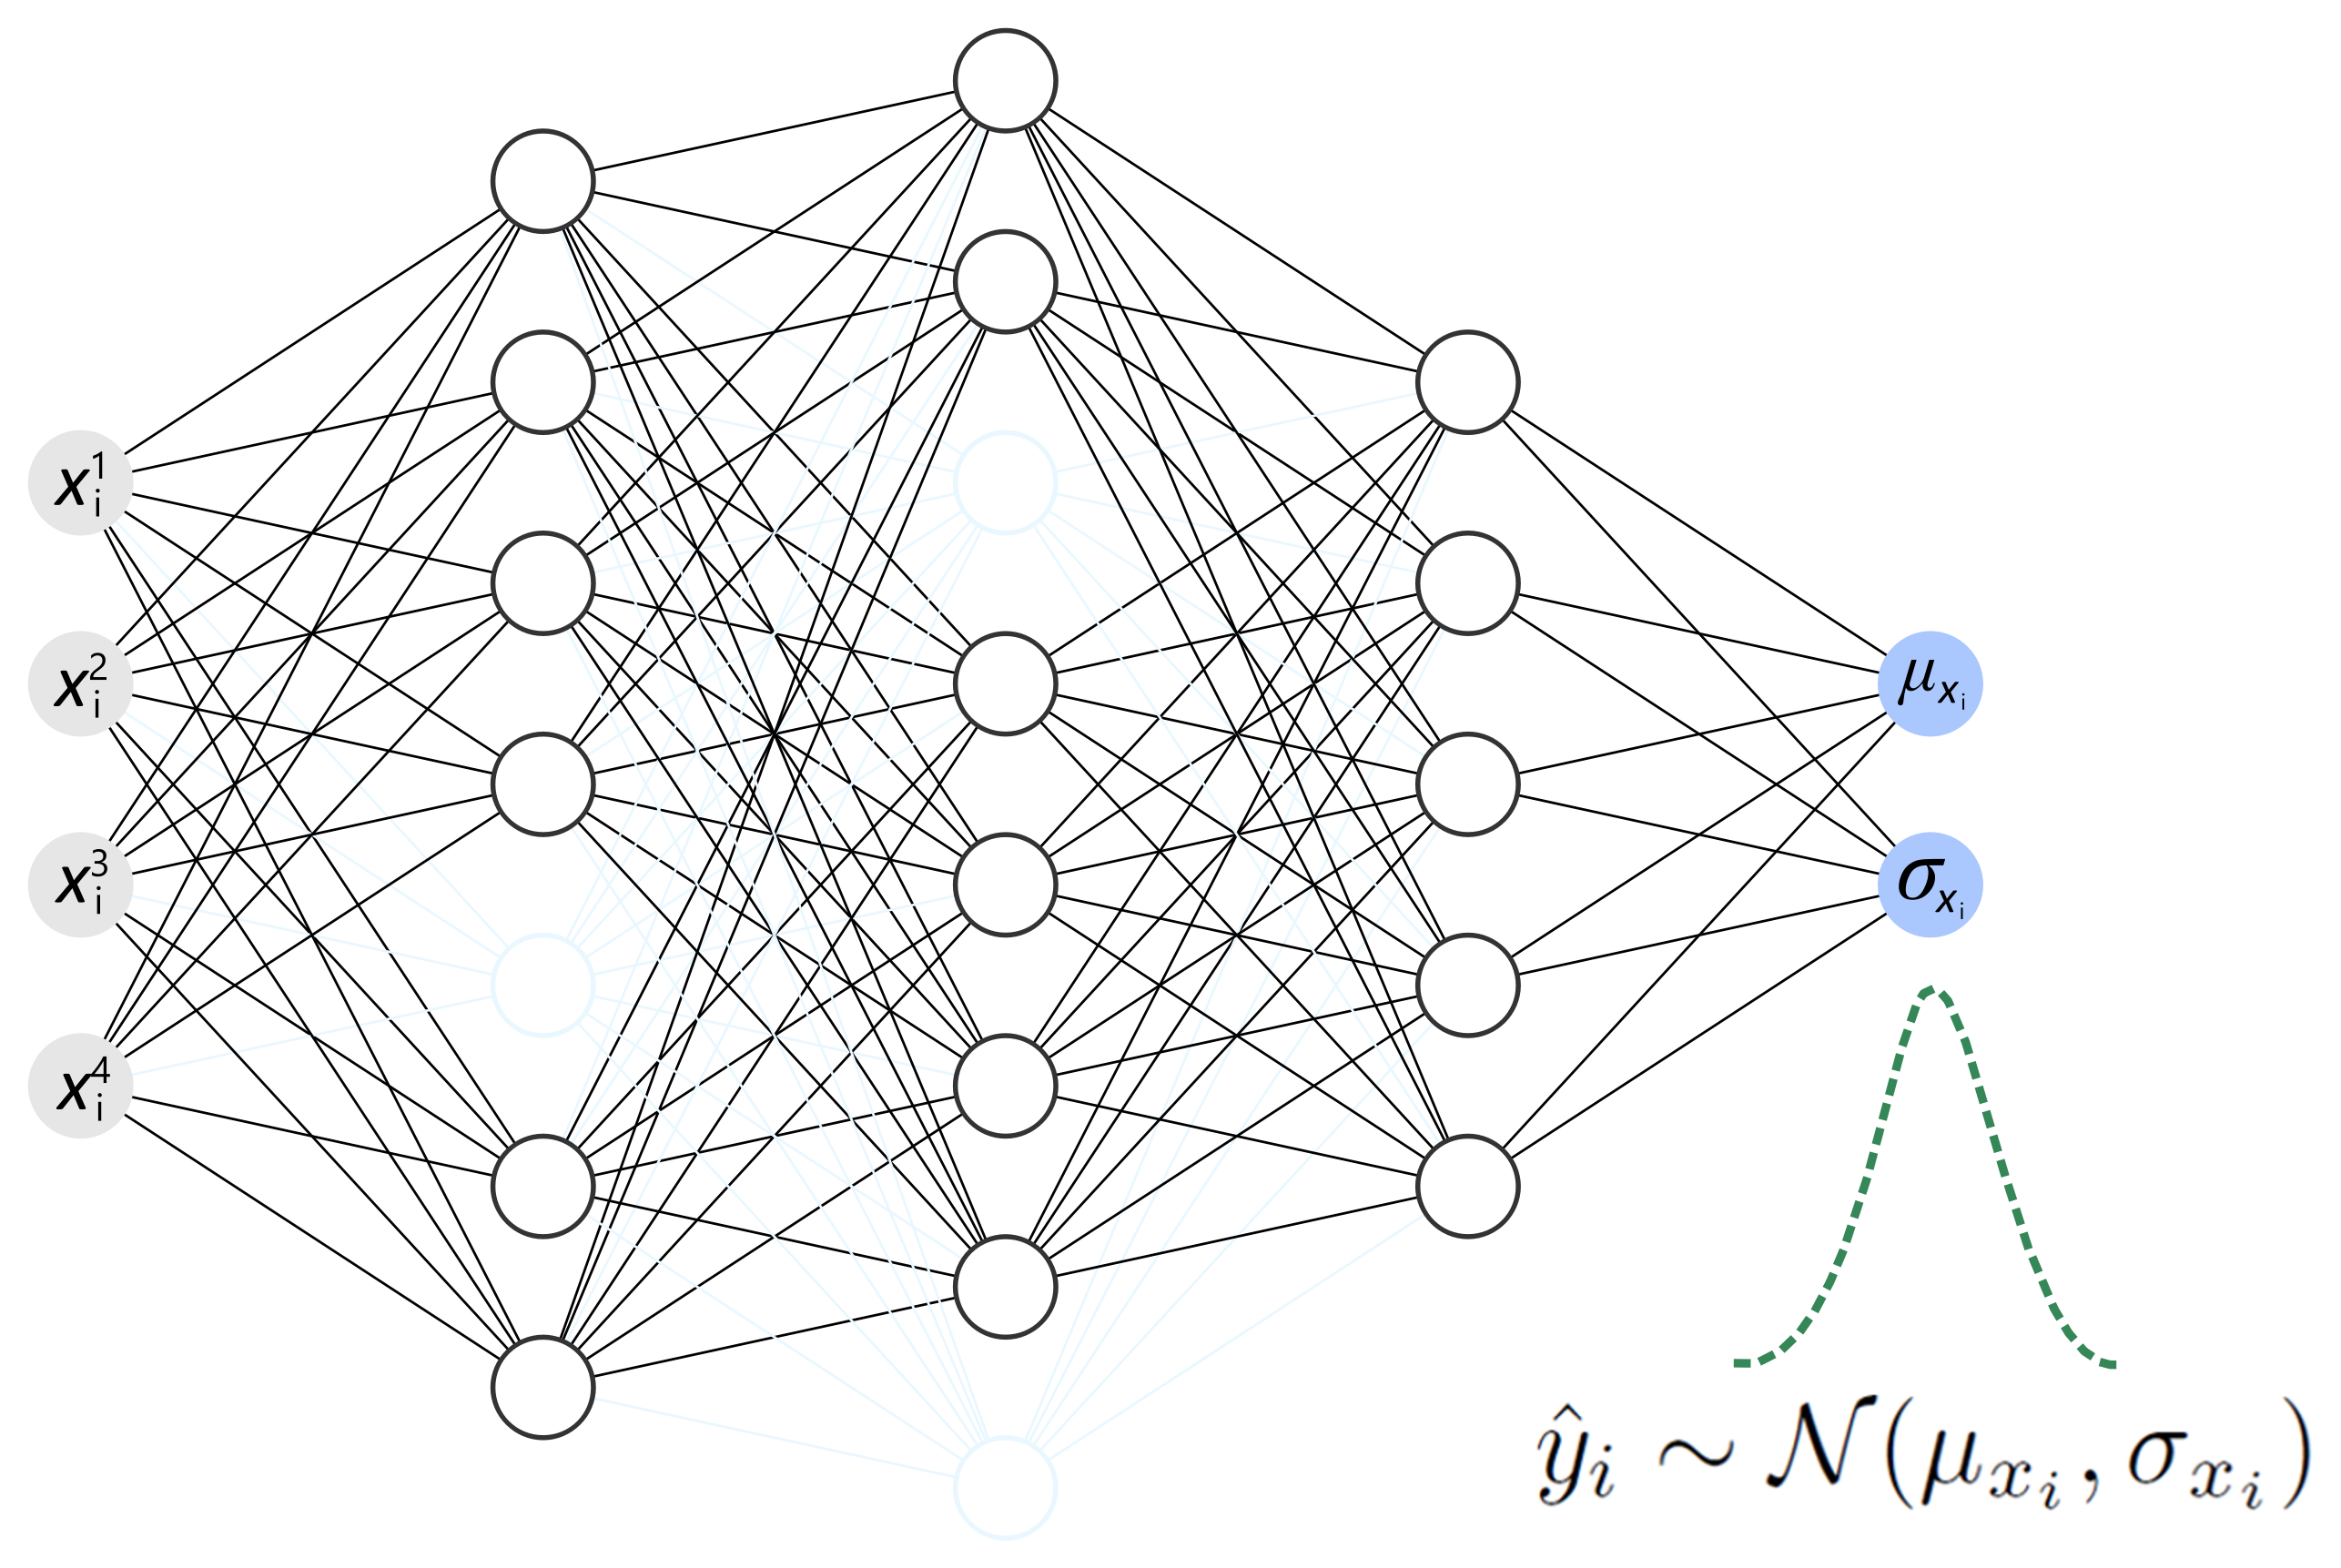
\includegraphics[width=0.7\linewidth]{baysurv_mcd.png}\\[-0.2em]
    {\scriptsize\textbf{MC dropout.}}\\[0.3em]
    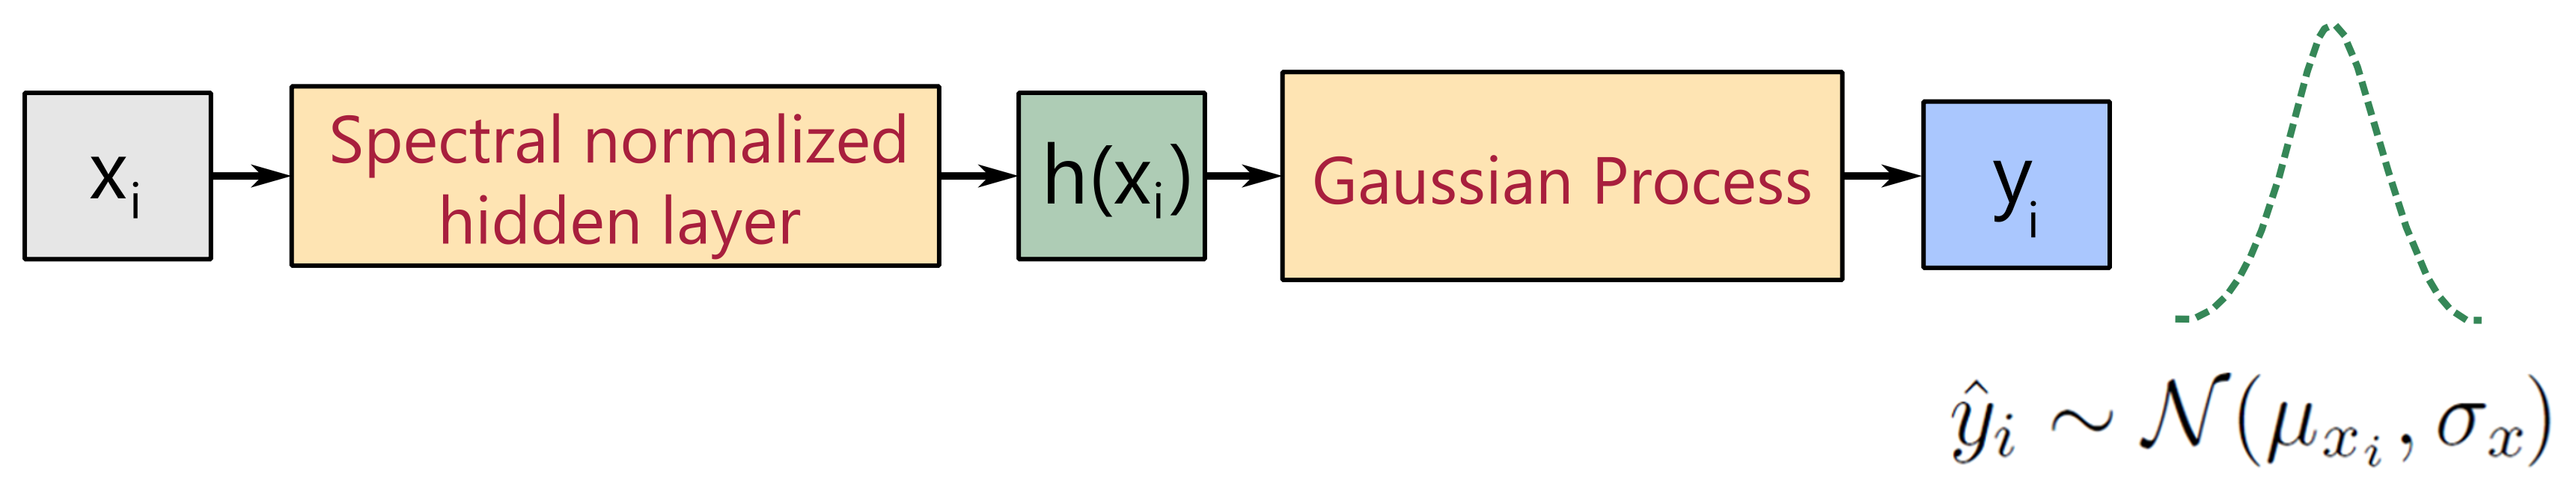
\includegraphics[width=0.9\linewidth]{baysurv_sngp.png}\\[-0.1em]
    {\scriptsize\textbf{SNGP.}}
    \figsource{Figures from Lillelund et al.~\cite{lillelund_efficient_2025}}
  \end{column}
\end{columns}
\end{frame}

\begin{frame}{MC dropout matches VI at half the cost}
\small Four datasets (METABRIC, SEER, SUPPORT, MIMIC-IV); D-calibrated if $p > 0.05$.

\centering
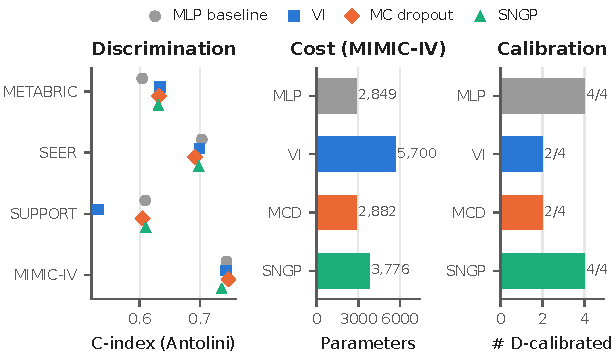
\includegraphics[width=0.82\linewidth]{plot_baysurv.pdf}
\figsource{Data from Lillelund et al.~\cite{lillelund_efficient_2025}. MC dropout shown with $p = 0.5$.}
\takeaway{MIMIC-IV: MC dropout 0.748 vs.\ VI 0.743 with half the parameters. SNGP: D-calibrated on 4/4.}
\end{frame}

\begin{frame}{Same median, different uncertainty}
\begin{columns}[c]
  \begin{column}{0.36\textwidth}
    \small
    One METABRIC patient, 1000 samples from the predictive distribution.
    \vspace{0.4em}
    \begin{itemize}
      \item Curve: mean $\E[S(t \mid \bm{x}_i)]$ with 90\% credible interval
      \item Histogram: predicted median times $\hat e_i$
    \end{itemize}
    \vspace{0.4em}
    True time 135 months.\\
    MC dropout: $\hat e_i = 122$\\
    VI: $\hat e_i = 128$ -- but far less certain.
  \end{column}
  \begin{column}{0.62\textwidth}
    \centering
    {\scriptsize\textbf{MC dropout} ($p = 0.5$)}\\
    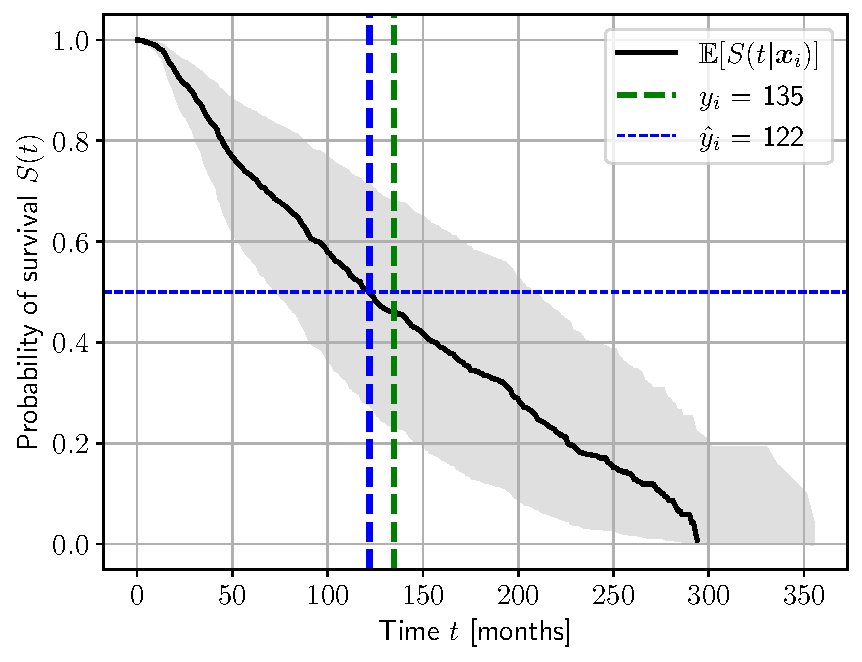
\includegraphics[width=0.49\linewidth]{metabric_cri.pdf}\hfill
    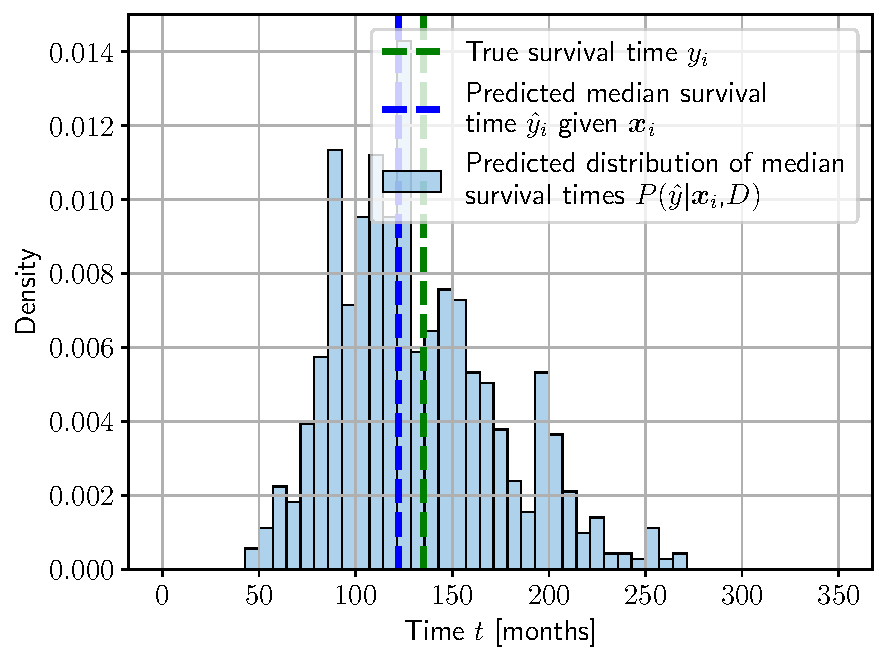
\includegraphics[width=0.49\linewidth]{metabric_cpd.pdf}\\[0.2em]
    {\scriptsize\textbf{Variational inference}}\\
    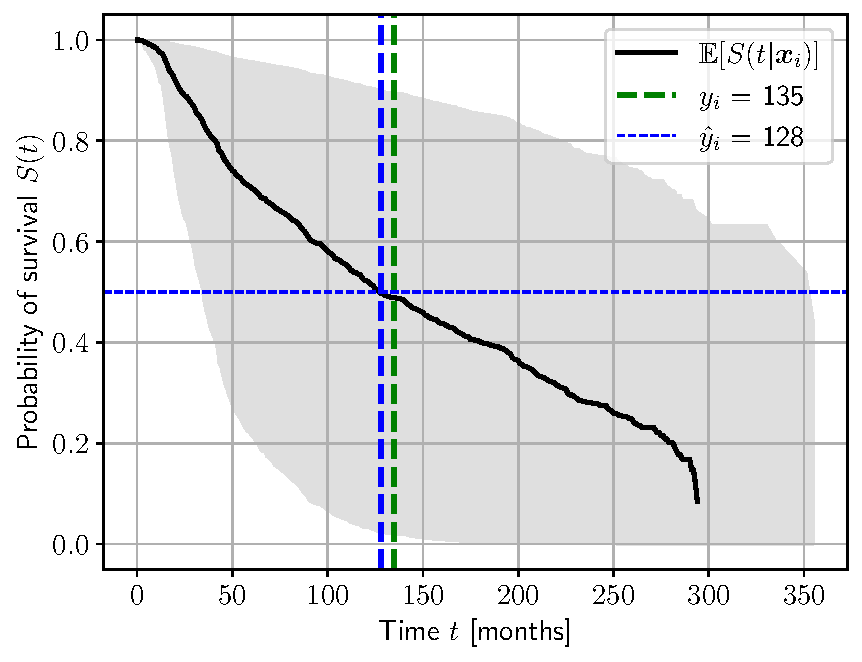
\includegraphics[width=0.49\linewidth]{metabric_cri_vi.pdf}\hfill
    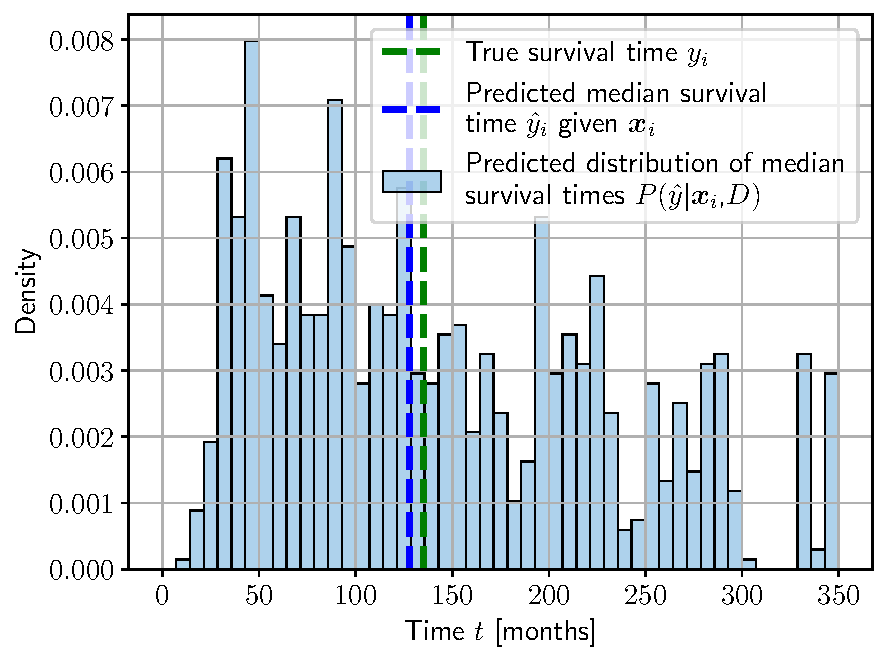
\includegraphics[width=0.49\linewidth]{metabric_cpd_vi.pdf}
    \figsource{Figures from Lillelund et al.~\cite{lillelund_efficient_2025}}
  \end{column}
\end{columns}
\vspace{0.3em}
{\footnotesize\textbf{Also in RQ1:} conformal prediction for TMJ involvement in children with JIA \cite{christensen_explainable_2024} -- the 90\% coverage holds on average, but early-stage cases are covered only 74\% of the time.\par}
\end{frame}

